\chapter{Database}

In this chapter we introduce the different methods we considered for a database representation and give reasons for final choice we made. Then we give a detailed description for our ER model.

%=======================================================================================
\section{Selection of the Database System}
For our database we considered NoSQL and SQL methods. We looked at different NoSQL solutions like MongoDB and CouchDB. Since nobody who was responsible for the database had experience with NoSQL wo chose to stick with the SQL approach. We  wanted to build a slim system. Therefore we first started to use SQLite. At this time we still used Python in the backend. Later in our project Python became no possibility for us anymore so moved to PHP. This also meant that we would change our SQLite system to MySQL, because one of our group members already had experience with this combination. After considering different possibilities we finally arrived back at the standard solution for a database. The advantages are that it is fast, well documented, the community is big and exists already for a long time so a lot of problems have been already discussed. On the other hand MySQL has so many functionalities that often it offers more complex solutions for less complicated problems. For example there is no support for constraints for values in tables in MySQL so that we had to use triggers which are handled way more complicated because they have way more funtionalities.
%=======================================================================================
\section{ER-Model}
    The figure \ref{fig:er_model} is the current state of our database visualized with an ER model.

	\begin{figure}[h!]
		\centering
			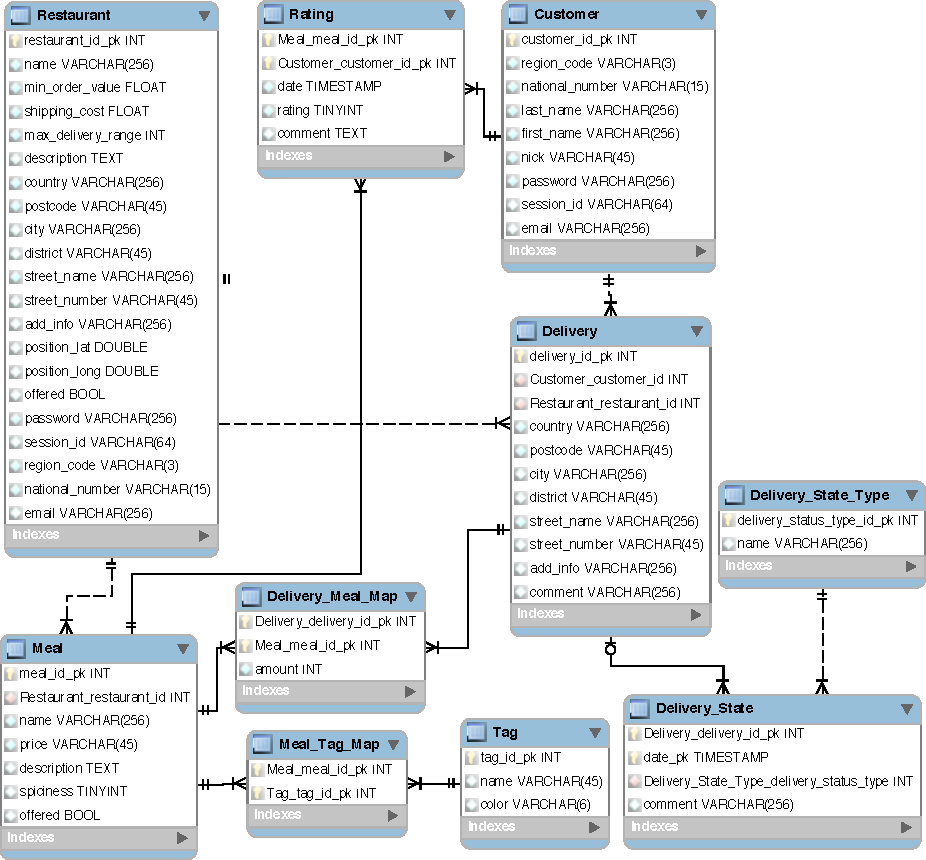
\includegraphics[scale=0.9]{content/graphics/er_model.pdf}
		\caption{ER model of our database.}
        \label{fig:er_model}
	\end{figure}

    An full description of the table will follow but first we explain the naming convention as well as the meaning of the colors in the ER model.

    \setdescription{itemsep=5pt,parsep=0pt,leftmargin=0.5cm, style=sameline}
    \begin{description}
        \item[attribute: (attribute name)] The attribute name is always written in lower case.
        item[primary key: (attribute name)\_pk] The attribute name concated with a '\_pk' at the end.
        \item[foreign key: (table name)\_(attribute name)] The table name is references the name of the table. Every first letter of every word in the table name is written in uppercase.
         \item[foreign key: (table name)\_(attribute name)\_pk] The foreign key name concated with a '\_pk' at the end.
    \end{description}
l
    The description for the colors of in the ER model.

    \setdescription{itemsep=5pt,parsep=0pt,leftmargin=0.5cm, style=sameline}
    \begin{description}
        \item[yellow] The attribute is a primary key.
        \item[red] The attribute is a foreign key which may not be NULL. The referenced primary key it identified by the name. 
        \item[lightblue] The attribute may not be NULL.
    \end{description}

    We will continue with a complete description of the database.

   \subsection{Customer}
    The Customer table saves the information of a customer.
    \setdescription{itemsep=5pt,parsep=0pt,leftmargin=0.5cm, style=sameline}
    \begin{description}
        \item[customer\_id\_pk: int(11)] The surrogate key of the customer by which the customer is identified.
        \item[region\_code: varchar(3)] The region code of the telephone number given by the customer.
        \item[national\_number: varchar(15)] The national number of the telephone number given by the customer.
        \item[last\_name: varchar(256)] The last name of the customer given by the customer
        \item[first\_name: varchar(256)] The first name of the customer given by the customer.
        \item[nick: varchar(45)] The nick name of the customer given by the customer. The nick name is unique.
        \item[password: varchar(256)] The password of the customer given by the customer.
        \item[session\_id: varchar(64)] The session id generated for the customer for each session.
        \item[email: varchar(256)] The email of the customer given by the customer.
    \end{description}

    \subsection{Delivery}
    \setdescription{itemsep=5pt,parsep=0pt,leftmargin=0.5cm, style=sameline}
    The Delivery table saves the information of a delivery
    \begin{description}
        \item[delivery\_id\_pk: int(11)] The surrogate key of the delivery by which the delivery is identified
        \item[Customer\_customer\_id: int(11)] The surrogate key of the customer who made delivery.
        \item[Restaurant\_restaurant\_id: int(11)] The surrogate key of the restaurant at which the delivery was made. 
        \item[country: varchar(256)] The country of the address the delivery should be delivered to.
        \item[postcode: varchar(45)] The postcode of the address the delivery should be delivered to.
        \item[city: varchar(256)] The city of the address the delivery should be delivered to.
        \item[district: varchar(45)] The district of the address the delivery should be delivered to.
        \item[street\_name: varchar(256)] The street name of the address the delivery should be delivered to.
        \item[street\_number: varchar(45)] The street number of the address the delivery should be delivered to.
        \item[add\_info: varchar(256)] Additional information of the address the delivery should be delivered to.
        \item[comment: varchar(256)] A comment for the restaurant which is added to the delivery by the user.
    \end{description}

    \subsection{Delivery\_Meal\_Map}
    The Delivery\_Meal\_Map table maps the delivery with the meal its included.
    \setdescription{itemsep=5pt,parsep=0pt,leftmargin=0.5cm, style=sameline}
    \begin{description}
        \item[Delivery\_delivery\_id\_pk: int(11)] The surrogate key of the delivery by which the delivery is identified.
        \item[Meal\_meal\_id\_pk: int(11)] The surrogate key of the meal by which the meal is identified wich is included in the delivery with the Delivery\_delivery\_id ID.
        \item[amount: int(11)] The number of the meals of the meal with the Meal\_meal\_id\_pk ID inclded in the delivery with the Delivery\_delivery\_id ID. The amount may not be negative.
    \end{description}

    \subsection{Delivery\_State}
    The Delviery\_State table maps a delivey to a delivery type.
    \setdescription{itemsep=5pt,parsep=0pt,leftmargin=0.5cm, style=sameline}
    \begin{description}
        \item[Delivery\_delivery\_id\_pk: int(11)] The surrogate key of the delivery by which the delivery is identified.
        \item[date\_pk: timestamp] The timestamp when the delivery status was applied.
        \item[Delivery\_State\_Type\_delivery\_status\_type: int(11)] The ID corresponding to 
        \item[comment: varchar(256)] A comment to this delivery status. Can be given by the restaurant or automatic by the system.
    \end{description}

    \subsection{Delivery\_State\_Type}
    The Delivery\_State\_Type is a static table which maps an ID to a delivery status type.
    \setdescription{itemsep=5pt,parsep=0pt,leftmargin=0.5cm, style=sameline}
    \begin{description}
        \item[delivery\_status\_type\_id\_pk: int(11)] The surrogate key which is used to save the delivery status type in the dynamic tables.
        \item[name: varchar(256)] The name of the delivery status type.
    \end{description}

    \subsection{Meal}
    The meal table represents a meal offered by an restaurant for customers.
    \setdescription{itemsep=5pt,parsep=0pt,leftmargin=0.5cm, style=sameline}
    \begin{description}
        \item[meal\_id\_pk: int(11)] The surrogate key of the meal by which the meal is identified.
        \item[Restaurant\_restaurant\_id: int(11)] The surrogate key of the restaurant which owns the meal.
        \item[name: varchar(256)] The name of the meal.
        \item[price: varchar(45)] The price of the meal. The price may not be negative.
        \item[Meal\_Category\_meal\_category\_id: int(11)] The surrogate key of the category of the meal.
        \item[description: text] The description of the meal.
        \item[spiciness: tinyint(3)] The value of spicinesss. It reaches from 0 to 3.
        \item[offered: tinyint(1)] A boolean value if the meal is still offered by the restaurant. 
    \end{description}

    \subsection{Meal\_Category}
    The Meal\_Category table is a static table which maps an ID to a category. Every dish can be categorized to one category. The categories are disjoint.
    \setdescription{itemsep=5pt,parsep=0pt,leftmargin=0.5cm, style=sameline}
    \begin{description}
        \item[meal\_category\_id\_pk: int(11)] The surrogate key which is used to save the meal category in the dynamic tables.
        \item[name: varchar(45)] The name of the meal category.
    \end{description}

    \subsection{Meal\_Tag\_Map}
    The Meal\_Tag\_Map table maps a number one tag to one Meal.
    \setdescription{itemsep=5pt,parsep=0pt,leftmargin=0.5cm, style=sameline}
    \begin{description}
        \item[Meal\_meal\_id\_pk: int(11)] The surrogate key of the meal the tag is mapped to.
        \item[Tag\_tag\_id\_pk: int(11)] The surrogate key of the tag the meal is mapped to.
    \end{description}

    \subsection{Rating}
    The Rating table represents a rating of a meal from a customer.
    \setdescription{itemsep=5pt,parsep=0pt,leftmargin=0.5cm, style=sameline}
    \begin{description}
        \item[Meal\_meal\_id\_pk: int(11)]  The surrogate key of the meal by which the meal is identified.
        \item[Customer\_customer\_id\_pk: int(11)] The surrogate key of the customer wich rated the meal.
        \item[date: timestamp] The date the rating was made.
        \item[rating: tinyint(4)] The rating of a dish. A rating reaches from 0 to 5.
        \item[comment: text] A comment added by the customer.
    \end{description}

    An additional constraint is that a customer cannot rate a meal before he ordered and received it.

    \subsection{Restaurant}
    \setdescription{itemsep=5pt,parsep=0pt,leftmargin=0.5cm, style=sameline}
    \begin{description}
        \item[restaurant\_id\_pk: int(11)] The surrogate key of the restaurant by which restaurant is identified.
        \item[name: varchar(256)] The name of the restaurant.
        \item[min\_order\_value: float] The minimum value a delivery from the restaurant has to be worth so it can be made. Tha value may not be zero.
        \item[shipping\_cost: float] The shipping cost of a delivery. The value may not be zero.
        \item[max\_delivery\_range: int(11)] The maximum range the customer can be away from the restaurant to make a delivery given in meters. The value may not be zero.
        \item[description: text] A description of the restaurant.
        \item[country: varchar(256)] The country of the address of the restaurant given by the restaurant.
        \item[postcode: varchar(45)] The country of the address of the restaurant given by the restaurant.
        \item[city: varchar(256)] The country of the address of the restaurant given by the restaurant.
        \item[district: varchar(45)] The district of the address of the restaurant given by the restaurant.
        \item[street\_name: varchar(256)]The street name of the address of the restaurant given by the restaurant.
        \item[street\_number: varchar(45)]The street number of the address of the restaurant given by the restaurant.
        \item[add\_info: varchar(256)] Additional information from the address given by the restaurant.
        \item[position\_lat: double] The latitude coordinate of the location of the address calculated by the system. The value may not be zero.
        \item[position\_long: double] The longitude coordinate of the location of the address calculated by the system. The value may not be zero.
        \item[offered: tinyint(1)] A boolean value if the restaurant is the still offering service.
        \item[password: varchar(256)] The password of the restaurant given by the restaurant.
        \item[session\_id: varchar(64)] The session id generated for the restaurant for each session.
        \item[email: varchar(256)] The email of the restaurant given by the restaurant.            
        \item[region\_code: varchar(3)] The region code of the telephone number given by the restaurant.
        \item[national\_number: varchar(15)] The national number of the telephone number given by the restaurant.
    \end{description}

    \subsection{Tag}
    The Tag table is a static table which maps an ID to a category. Every dish can be tagged with several tags by the restaurant. A tag describes a feature of a dish.
    \setdescription{itemsep=5pt,parsep=0pt,leftmargin=0.5cm, style=sameline}
    \begin{description}
        \item[tag\_id\_pk: int(11)] The ID which is used to save the tag in the dynamic tables.
        \item[name: varchar(45)] The name of the tag.
        \item[color: varchar(6)] The color code of the color used to represent the tag in the frontend.
    \end{description}

    \section{Static tables}
    In this section we present the tables which are not used for inserts. Instead saving a string repeatedly in intensively used tables we just save an ID and use a static table for mapping this ID to a string. We present the values of the static tables. The Tag table: 
    \begin{center}
        \begin{tabular}{|l|l|l|l|}
            \hline
            tag\_id\_pk & meaning & color code & color\\ \hline
            1 & Vegetarian & \#22c13e & light green \\ \hline
            2 & Vegan & \#195805 & dark green \\ \hline
            3 & Pork & \#f97990	& pink \\ \hline
            4 & Cold & \#73b9c1 & light blue \\ \hline
            5 & Kosha & \#6c1547 & purple \\ \hline
        \end{tabular}
    \end{center}
    The Delivery\_State\_Type table: 
    \begin{center}
        \begin{tabular}{|l|l|p{5cm}|}
            \hline
            delivery\_status\_type\_id\_pk & name & meaning \\ \hline
            1 & PENDING & The delivery was ordered by a customer but the restaurant has not seen the delivery yet. \\ \hline
            2 & PROCESSING & The restaurant has seen and accepted the delivery and will proceed with it. \\ \hline
            3 & INDELIVERY & The restaurant sended the delivery out. \\ \hline
            4 & DONE & The delivery has been delivered. \\ \hline
        \end{tabular}
    \end{center}

    \section{Views}
    This is a list of Views we use. We basically just use them to avoid the inner joins with the static tables in every request.
    \setdescription{itemsep=5pt,parsep=0pt,leftmargin=0.5cm, style=sameline}
    \begin{description}
        \item[Delivery\_State\_View] Joins the Delivery\_State with Delivery\_State\_Type together.
        \item[Delivery\_View] Joins the Delivery with Delivery\_State together
    \end{description}
